\documentclass[a4paper,11pt]{article}
\input{/home/tof/Documents/Cozy/latex-include/preambule_lua.tex}
\newcommand{\showprof}{show them}  % comment this line if you don't want to see todo environment
\fancyhead[L]{Andy Warhol - les fonctions}
\newdate{madate}{10}{09}{2020}
\fancyhead[R]{Première - NSI} %\today
\fancyfoot[L]{~\\Christophe Viroulaud}
\fancyfoot[C]{\textbf{Page \thepage}}
\fancyfoot[R]{\includegraphics[width=2cm,align=t]{/home/tof/Documents/Cozy/latex-include/cc.png}}
\usepackage{tikz}
\begin{document}
\begin{Form}
\section{Problématique}
Artiste américain mort en 1987, Andy Warhol était un  des principaux représentants du \emph{pop art}.	Le \emph{dyptique de Marylin Monroe} réalisé en 1962 est une de ses œuvres célèbres. Il contient cinquante fois la même image de l'actrice mais avec un travail des couleurs différent.
\begin{figure}[!h]
\centering
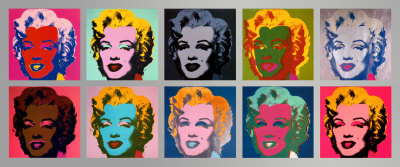
\includegraphics[width=8cm]{ressources/marylin.jpg}
\captionof{figure}{Dyptique de Marylin Monroe}
\label{monroe}
\end{figure}
\begin{center}
\shadowbox{\parbox{14cm}{\centering Peut-on réaliser un programme qui reproduit le concept de cette œuvre?}}
\end{center}
\section{Manipuler une image}
\subsection{Présentation de la bibliothèque}
La bibliothèque \emph{Pillow} est un outil pour faciliter la manipulation des images.
\begin{activite}
Expliquer le rôle de chaque ligne du code \ref{pil}.
\end{activite}
\begin{code}[!h]
\begin{lstlisting}
from PIL import Image

originale = Image.open("../ressources/joconde.jpg")
ligne, colonne = originale.size
\end{lstlisting}
\captionof{code}{La bibliothèque Pillow}
\label{pil}
\end{code}
\subsection{Couleurs d'une image}
Une image peut être vue comme un tableau de pixels de \emph{l} lignes et \emph{c} colonnes. Chacun de ces points de l'image code une couleur.\\
Pour obtenir une grande gamme de couleurs, le principe de la synthèse additive est utilisé. En combinant une quantité de Rouge, Vert, Bleu (RGB en anglais) il est possible de créer une palette importante. 
\begin{figure}[!h]
\centering

\includegraphics[width=3cm]{ressources/additive.jpg}
\captionof{figure}{Synthèse additive}
\label{additive}
\end{figure}

Chaque pixel peut ainsi être vu comme un tuple (Rouge, Vert, Bleu), chaque composante étant codé sur \emph{8 bits}.
\begin{activite}
\begin{enumerate}
\item Combien de valeurs peut prendre chaque composante?
\item Calculer alors le nombre de couleurs qu'il est possible de coder.
\end{enumerate}
\end{activite}
\subsection{Principe de la modification}
Pour modifier l'image originale nous allons appliquer le protocole ci-après.\\
Pour chaque pixel:
\begin{itemize}
\item récupérer le tuple des trois composantes,
\item créer un nouveau pixel en appliquant la transformation désirée,
\item poser le nouveau pixel à la même position dans l'image.
\end{itemize}
\begin{activite}
\begin{enumerate}
\item À l'aide de la documentation de la bibliothèque (\url{https://tinyurl.com/y3g95hj3}) récupérer et afficher le tuple du pixel de coordonnées (10,10).
\item Créer un nouveau pixel qui ne conserve que la composante rouge de ce pixel.
\end{enumerate}
\end{activite}
\section{Première œuvre d'art}
\begin{activite}
\begin{enumerate}
\item En s'aidant de la documentation, \emph{créer une copie} de l'image originale.
\item Écrire un programme qui charge l'image originale, la transforme en ne conservant que la composante rouge et affiche cette nouvelle version.
\end{enumerate}
Le code \ref{new} crée une nouvelle image vide deux fois plus grande et haute que l'originale.
\begin{center}
\begin{lstlisting}
img = Image.new('RGB', (ligne*2,colonne*2))
\end{lstlisting}
\captionof{code}{Une image vide}
\label{new}
\end{center}
\begin{enumerate}[resume]
\item En s'aidant de la documentation, \emph{coller} l'image rouge en haut à droite de \emph{img}.
\item Créer trois variations de l'image originale et les placer aux trois autres positions de \emph{img}. 
\end{enumerate}
\end{activite}
\section{Améliorer le programme}
\begin{commentprof}
Si nous voulions créer une image avec cinquante variations de couleurs, il deviendrait très long. Pourtant on constate que de grandes portions de codes se ressemblent. 
\end{commentprof}
\subsection{Les fonctions mathématiques}
En première approche, on peut voir une fonction mathématique comme une boîte réutilisable à qui on donne une valeur, qui effectue les opérations pour laquelle elle a été créée et qui nous renvoie le résultat.
\begin{figure}[!h]
\centering
\begin{tikzpicture}
\node(x) at (-4,0) {4};
\node[draw,fill=gray!10,minimum height=1.5cm] (f) at (0,0) {$x^2+3×x^3+\sqrt{16×x}-\dfrac{x^5}{10}$};
\node(res) at (4,0) {113,6};

\draw[->,>=latex] (x) -- (f);
\draw[->,>=latex] (f) -- (res);
\end{tikzpicture}
\captionof{figure}{La fonction $f(x)$ calcule et renvoie la valeur}
\label{fonction}
\end{figure}
\subsection{Les fonctions en programmation}
Le même principe est appliqué en programmation. En Python, la syntaxe est la suivante:
\begin{code}[!h]
\begin{lstlisting}
def ma_fonction(x):
	f = x**2 + 3*x**3 + sqrt(16*x) - x**5/10
	return f
\end{lstlisting}
\captionof{code}{Définir une fonction}
\label{def}
\end{code}

Les mots clefs à retenir:
\begin{itemize}
\item \textbf{def} annonce qu'on définit une fonction qui a pour nom \emph{ma\_fonction} dans l'exemple.
\item \textbf{return} précise qu'on sort de la fonction ici et qu'on \emph{renvoie} la valeur de la variable \emph{f} ici.
\end{itemize}
La fonction est crée, il faut maintenant l'utiliser dans le programme principal.
\begin{lstlisting}
print(ma_fonction(4))
\end{lstlisting}
Dans le code \ref{def} on remarque que la fonction possède un \textbf{paramètre} noté \emph{x}. Dans le programme principal, on \emph{passe} l'\textbf{argument} 4 à la fonction. Cette dernière remplacera chaque occurrence de \emph{x} par 4.
\begin{activite}
\begin{enumerate}
\item Tester ma\_fonction avec plusieurs valeurs de x.
\item Écrire une fonction \textbf{maxi(x, y)} qui demande deux paramètres \emph{x} et \emph{y} et qui renvoie la plus grande des deux valeurs.
\end{enumerate}
\end{activite}
\subsection{Application à l'œuvre d'art}
\begin{commentprof}
Les intérêts de créer une fonction sont multiples:
\begin{itemize}
\item créer des outils réutilisables
\item rendre le code plus lisible
\end{itemize} 
\end{commentprof}
Le programme pour réaliser l'œuvre d'art présente des portions de code similaires. 
\begin{activite}
\begin{enumerate}
\item Créer une fonction \textbf{img\_filtree(image, R, V, B)} qui prend une \emph{image} comme argument ainsi que trois nombres, \emph{R, V, B} compris entre 0 et 1. Ces valeurs représentent les proportions de Rouge, Vert et Bleu. La fonction renverra l'image filtrée.
\item Utiliser alors cette fonction et écrire un nouveau programme pour créer l'œuvre d'art.
\end{enumerate}
\end{activite}
\end{Form}
\end{document}